\documentclass{standalone}
\usepackage{tikz}
\usepackage{pgfplots}
\pgfplotsset{compat=1.18}

\begin{document}

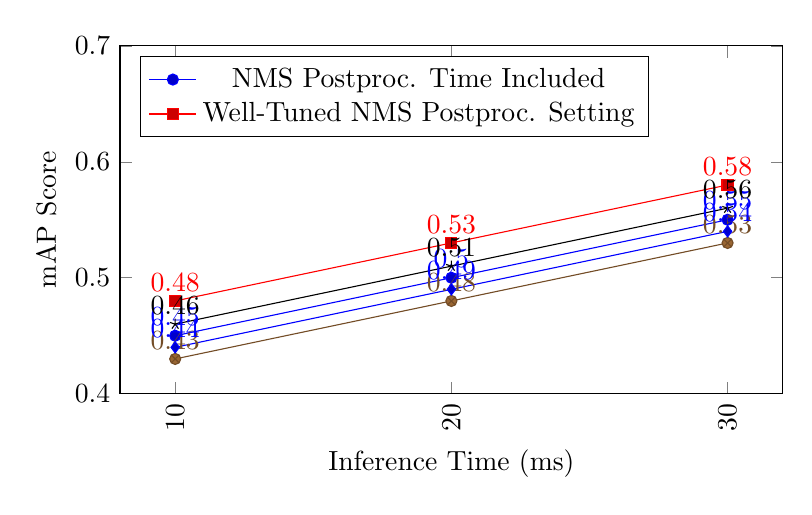
\begin{tikzpicture}
    \begin{axis}[
        width=10cm,
        height=6cm,
        xlabel={Inference Time (ms)},
        ylabel={mAP Score},
        ymin=0.4,
        ymax=0.7,
        xtick=data,
        x tick label style={rotate=90},
        nodes near coords,
        nodes near coords align={vertical},
        legend pos=north west,
        legend entries={Model A, Model B, Model C, Model D, Model E}
    ]
        
        % Data points for each model
        \addplot coordinates {(10, 0.45) (20, 0.50) (30, 0.55)};
        \addlegendentry{NMS Postproc. Time Included}
        \addplot coordinates {(10, 0.48) (20, 0.53) (30, 0.58)};
        \addlegendentry{Well-Tuned NMS Postproc. Setting}
        
        % Other models data points
        \addplot coordinates {(10, 0.43) (20, 0.48) (30, 0.53)};
        \addplot coordinates {(10, 0.46) (20, 0.51) (30, 0.56)};
        \addplot coordinates {(10, 0.44) (20, 0.49) (30, 0.54)};
        
    \end{axis}
\end{tikzpicture}

\end{document}